\chapter{Some SDP experiments} \label{chap:sdpExp}
\minitoc
\vfill
%\epigraph{test epigraph...}{\textit{in a book \\ by an author}}
\noindent
\begin{minipage}[c]{0.3\linewidth}
\includegraphics[width=\textwidth]{experiments}
\end{minipage}
\hfill
\begin{minipage}[c]{0.7\linewidth}
\begin{abstract}
In the last chapter, we have proved that the System Dimensioning Problem {\SDP} can be approached using an integer linear program.
Although a polynomial sub case of the {\SDP} has been highlighted, the global problem complexity is still unknown.
It rises the question of an acceptable computing time and resources according to our industry context.
Can the program deal with real instances, or at least realistic case studies?
We propose in this chapter to evaluate the problem from a computational perspective.
\end{abstract}
\end{minipage}

\newpage
\section{Introduction}
The lack of available real carsharing demand data prevents us from a meaningful confrontation between an actual operating carsharing system and an optimal system dimensioning configuration computed from the linear program solution.

\bigskip
We presented in Chapter \ref{chap:backAndPb} a random data generator that has been developed especially to cope with that lack.
It defines a specific time environment, generates a random set of stations with settable maximum capacities and a realistic set of carsharing demands from origins to destinations during a typical weekday.

\bigskip
This chapter focuses on computational experiments based on the random data generator.
It explores several computing aspects of the linear program, from the maximum problem size the program can solve to observed solver computation times.
Generator parameter values will be specified at the beginning of each experiment.
For more details on the random data generator, see Section \ref{csgeneratorDescription} page \pageref{csgeneratorDescription}.

\bigskip
This chapter is organize as follow.
Section \ref{sec:firstExperiments} gives some discussion about computation times and solutions analysis of small instances, based on generated data.
A 3-dimensional Pareto frontier is especially presented.
Section \ref{sec:relocExperiments} is dedicated to scalability experimentations, particularly the solver's performance when the problem increases in size.

\section{First experiments and scalability} \label{sec:firstExperiments}
\subsection{Experimental context}
In this first section, all experimental results were made using an Intel(R) Core(TM) i3-3227U CPU running at $1.9$GHz. The linear programs were expressed using the AMPL format \cite{ampl_webPage} and numerical results were obtained using the open-source solver GLPK v4.52 \cite{glpk_webPage}.

\bigskip
The choice of GLPK instead of a commercial solver is mainly motivated by our industrial context.
The will to transfer easily our methodology and tools in an industrial environment initially led us to use an open-source solver.
Although the solutions we obtained with GLPK were quite good, some hard limitations related to the program build time lead us to use later on CPLEX, a more flexible and powerfull solver.

\subsection{3-pareto fontier}
First experiment aims at assessing solver computation times of ``small'' SDP instances.
Considering $\nbStations = 10$ stations, $\nbTimeSteps = 144$ time-steps and $\nbDemands = 500$ demands, we collected program building time and solver computation times of $30$ random instances.
We assumed here that the system could be balanced using vehicle relocation operations at any time-step in $\timeStepSet$ (\ie $\relocTimeStepSet = \timeStepSet$).

\bigskip
For those fixed SDP inputs, the corresponding TEG has:
\begin{itemize}
\item $|\tegNodeSet| = \nbStations \cdot \nbTimeSteps = 10 \cdot 144 = \np{1440}$ nodes, and
\item $|\tegArcSet| = \nbStations \cdot \nbTimeSteps + \nbDemands + |\relocTimeStepSet| \cdot \nbStations \cdot (\nbStations - 1) = (10 \cdot 144) + 500 + (144 \cdot 10 \cdot 9) = \np{14900}$ arcs. This value is actually an upper-bound of the number of arc since $\nbDemands$ is interpreted by the generator as $\sum_{a \in \tegArcSet_2} u(a)$, which potentially lead to the situation where $|\tegArcSet_2| < \nbDemands$.
\end{itemize}

For each random instance, the solver computation determines the maximum number of carsharing demands the system is able to satisfy according to different upper bound of relocation operations (R) and the number of vehicles (C).
After having tested some empirical values of R and C, we observed that setting both of them to $\{0, 10, \cdots, 80\}$ produce the most representative results.
Based on each single instance, a total of $9 \times 9 = 81$ linear programs are then solved (9 values for both R and C).
Table \ref{table:computationTimes} presents the average computation time $\mu$ and the standard deviation $\sigma$ for both integer linear program ILP and its relaxation to linear program LP.
The minimal and maximal computation time values are also specified.
Note that the linear program in this experiment contains $|\tegArcSet| = \np{14900}$ variables, and  $1442$ constraints.

\begin{table}[t]
\renewcommand{\arraystretch}{2.3}
\centering
\begin{tabularx}{.8\linewidth}{|c|*{5}{>{\centering \arraybackslash}X|}}
\cline{2-5}
\multicolumn{1}{c|}{} & $\mu$ & $\sigma$ & $\min$ & $\max$ \\
\hline
LP  & $0,56$ & $0,25$ &	$<0,01$ &  $1,17$ \\
ILP & $1,93$ & $1,86$ &	$<0,01$ & $16,77$ \\
\hline
\end{tabularx}
\caption{GLPK computation times in seconds for small instances.}
\label{table:computationTimes}
\end{table}

\bigskip
The first observation is that computation times remain quite low, in the order of a half-second for LPs and two seconds for ILPs.
The major part is taken by the building of the mathematical program which takes $34$ seconds (mostly  by the conservation law's constraints) regardless of which model is built.
Maintaining the same problem size, further experiments with CPLEX reduce this building time to a half-second.

\bigskip
Secondly, when the solver runs the LP model, almost $8$ problems under $81$, exactly $7,66$ on average over the $30$ generated instances, admit a non-integer value of the objective function.
This result represents almost $10\%$ of all instances.
However, every time we get a non-integer optimal value $LP^*$, the integer one $ILP^*$ has always the same integer part.
In other words, we observed in all cases that $ILP^* = \lfloor LP^* \rfloor$.

%\bigskip
%Hence it comes that we conjecture the existence of an integer optimal solution for LP and that the difference between the two criteria values comes from rounding errors > peut etre changer la conclusion.

\begin{figure}[t]
\centering
\includegraphics[width=.8\linewidth]{result_parteo_frontier}
\caption{A coloured layer 3-dimensional Pareto frontier for a particular instance with $10$ stations and $500$ demands.}
\label{fig_pareto}
\end{figure}

\bigskip
Plotting the maximal number of satisfied demands found by the solver regarding different couple values ${(R, C) \in \{0, 10, \dots, 80\}^2}$, allow us to confirm that the number of vehicle relocation operations is in opposition with the number of vehicles.
Figure \ref{fig_pareto} shows a 3-dimensional Pareto frontier made of $81$ points for a particular problem instance.
The coloured layers correspond to different demand satisfaction levels.
The yellow level for instance denotes a satisfaction level between $60$\% and $80$\%, whereas the green level stands for the maximal satisfaction level ($100$\%).

\bigskip
In this specific case, the tradeoff between the two criteria is well highlighted.
The more the number of vehicle relocation operations, the less the number of vehicle needed to run the system.
For instance, $70$ vehicle relocation operations with $50$ vehicles allow to capture all $500$ demands.
Maintaining the same service quality (satisfying all the demands in this case) while decreasing the number of vehicle relocation operations imply increased at the same time the number of vehicles.
Thus, $70$ vehicles are needed if the system is balanced with at most $70$ vehicles relocation operations.
This confirms that the two criteria are in opposition and that there exists a tradeoff area between them.

\subsection{Scalability study}
Solving small instances of the system dimensioning problem with a linear programming approach is not a problem in itself.
Even with an open-source solver like GLPK, the obtained computation times remain in a range of a few seconds and are therefore reasonable.
However, the high time needed to build the programs, due to the graph density, is certainly a challenge we have to handle.

\bigskip
As observed previously, its most important part comes from the formal expression of the conservation law's constraints, probably mismanaged by the solver.
This second experimentation focuses on the problem scalability when the problem is growing in size.
More especially, we investigate the overall program building time evolution when the number of stations and the number of time-steps increase.

\bigskip
In the first place, we studied systems where the number of stations and the number of time-steps respectively belong to $\{10, 20, \dots, 50\}$ and $\{72, 144, 288\}$, which corresponds to time-step intervals of $20$, $10$ and $5$ minutes.
Each measure is obtained from a single instance since the time needed to build the model only depends on the size of the time extended graph.
For the record, Table \ref{table:graphDensities} presents graph densities for the different problem's sizes.
First numerical results, obtained with GLPK, are presented in Table \ref{table:generationTimesGLPK} and plotted in Figure \ref{plot:buildingTimes}.

\begin{table}[t]
\renewcommand{\arraystretch}{1.8}
\centering
\begin{tabularx}{.9\linewidth}{|c|*{5}{>{\centering \arraybackslash}X|}}
\hline
\backslashbox{$\nbTimeSteps$~}{$\nbStations$~} & $10$ & $20$ & $30$ & $40$ & $50$\\

\hline
\multirow{2}{*}{$72$} & \multirow{2}{*}{$14$} & \multirow{2}{*}{$59$} & $138$ & $147$ & $310$\\
& & & $\approx 2'30$ & $\approx 3'$ & $\approx 5'$\\

\hline
\multirow{2}{*}{$144$} & \multirow{2}{*}{$53$} & $234$ & $343$ & $632$ & $1437$\\
& & $\approx 4'$ & $\approx 5'30$ & $\approx 10'30$ & $\approx 24'$\\

\hline
\multirow{2}{*}{$288$} & $211$ & $997$ & $1417$ & $2481$ & $4735$\\
& $\approx 2'30$ & $\approx 16'30$ & $\approx 23'30$ & $\approx 41'30$ & $\approx 1$h$20'$\\

\hline
\end{tabularx}
\caption{Generation time in seconds obtained with GLPK according to the problem's size (number of stations and times-steps).}
\label{table:generationTimesGLPK}
\end{table}

\begin{table}[t]
\renewcommand{\arraystretch}{1.8}
\centering
\begin{tabularx}{.9\linewidth}{|c|*{5}{>{\centering \arraybackslash}X|}}
\hline
\backslashbox{$\nbTimeSteps$~}{$\nbStations$~} & $10$ & $20$ & $30$ & $40$ & $50$\\

\hline
\multirow{2}{*}{$72$} & $|\tegNodeSet| = \np{720}$ & $\np{1440}$ & $\np{2160}$ & $\np{2880}$ & $\np{3600}$\\
& $|\tegArcSet| = \np{7700}$ & $\np{29300}$ & $\np{65300}$ & $\np{115700}$ & $\np{180500}$\\

\hline
\multirow{2}{*}{$144$} & $\np{1440}$ & $\np{2880}$ & $\np{4320}$ & $\np{5760}$ & $\np{7200}$\\
& $\np{14900}$ & $\np{58100}$ & $\np{130100}$ & $\np{230900}$ & $\np{360500}$\\

\hline
\multirow{2}{*}{$288$} & $\np{2880}$ & $\np{5760}$ & $\np{8640}$ & $\np{11520}$ & $\np{14400}$\\
& $\np{29300}$ & $\np{115700}$ & $\np{259700}$ & $\np{461300}$ & $\np{720500}$\\

\hline
\end{tabularx}
\caption{Graph densities according to the problem's size (number of stations and times-steps). In each cell, the above number stands for the number of nodes while the bellow one stands for the number of arcs.}
\label{table:graphDensities}
\end{table}

\begin{figure}[t]
\centering
\begin{subfloat}[]{\label{plot:graphdensities}
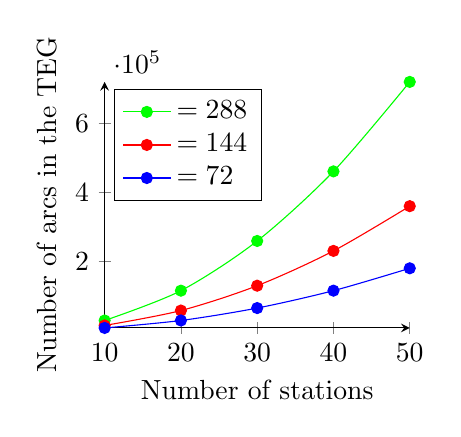
\begin{tikzpicture}
\begin{axis}[
width=.45\linewidth,
xlabel=Number of stations,
ylabel=Number of arcs in the TEG,
legend pos=north west,
legend cell align=left,
axis x line=bottom,
axis y line=left,
]

\addplot[smooth,mark=*,color=green] plot coordinates {
(10,29300)
(20,115700)
(30,259700)
(40,461300)
(50,720500)
};
\addlegendentry{$\nbTimeSteps = 288$}

\addplot[smooth,mark=*,color=red] plot coordinates {
(10,14900)
(20,58100)
(30,130100)
(40,230900)
(50,360500)
};
\addlegendentry{$\nbTimeSteps = 144$}

\addplot[smooth,mark=*,color=blue] plot coordinates {
(10,7700)
(20,29300)
(30,65300)
(40,115700)
(50,180500)
};
\addlegendentry{$\nbTimeSteps = 72$}

\end{axis}
\end{tikzpicture}}
\end{subfloat}
\hfill
\begin{subfloat}[]{\label{plot:buildingTimes}
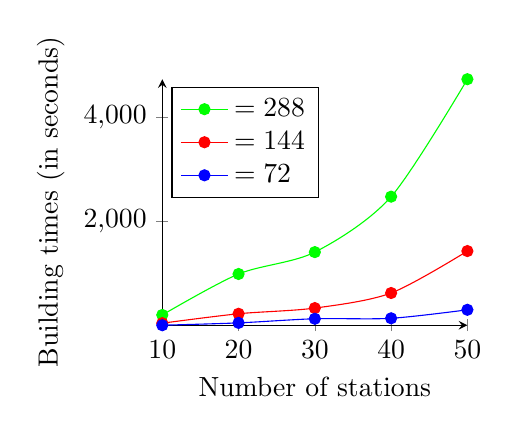
\begin{tikzpicture}
\begin{axis}[
width=.45\linewidth,
xlabel=Number of stations,
ylabel=Building times (in seconds),
legend pos=north west,
legend cell align=left,
axis x line=bottom,
axis y line=left,
]

\addplot[smooth,mark=*,color=green] plot coordinates {
(10,211)
(20,997)
(30,1417)
(40,2481)
(50,4735)
};
\addlegendentry{$\nbTimeSteps = 288$}

\addplot[smooth,mark=*,color=red] plot coordinates {
(10,53)
(20,234)
(30,343)
(40,632)
(50,1437)
};
\addlegendentry{$\nbTimeSteps = 144$}

\addplot[smooth,mark=*,color=blue] plot coordinates {
(10,14)
(20,59)
(30,138)
(40,147)
(50,310)
};
\addlegendentry{$\nbTimeSteps = 72$}

\end{axis}
\end{tikzpicture}}
\end{subfloat}
\caption{Similar curve shape for TEG densities \protect\subref{plot:graphdensities}\\ and GLPK building times \protect\subref{plot:buildingTimes}.}
\label{fig:plotsGraphDensitiesBuildingTimes}
\end{figure}

\bigskip
We observed that the generation time grows linearly following the number of arcs in the time extended graph.
Note that for the biggest instance ($\nbStations = 50$ stations and $\nbTimeSteps = 288$ time-steps) GLPK founds a relaxed optimal solution within $1'20$ minute and an integer optimal solution within $1'30$ minute, while the number of arcs stands around $\np{700000}$.
Moreover, this linear relation is consolidated by the correlation coefficient (Pearson product-moment correlation coefficient) between GLPK generation time and the number of arcs in the graph standing at $95,9\%$.
This result can be easily noticeable in Figure \ref{fig:plotsGraphDensitiesBuildingTimes} and looks coherent since the size of the linear model and the number of variables are both in $\Theta(|\tegArcSet|)$.

\bigskip
After having developed the optimization model with CLPEX, we replicated the building time experiment.
Numerical results are shown in Table \ref{table:generationTimesCPLEX}.
This time, program generation time values are much more smaller.
The reduction factor varies from $304$ for instances with $\nbStations = 10$ and $\nbTimeSteps = 72$ to $\np{2437}$ for instances with $\nbStations = 20$ and $\nbTimeSteps = 288$.
The largest program is build within 6 seconds with CPLEX compared to $1$ hour and $20$ minutes for GLPK.

\begin{table}[t]
\renewcommand{\arraystretch}{1.8}
\centering
\begin{tabularx}{.9\linewidth}{|c|*{5}{>{\centering \arraybackslash}X|}}
\hline
\backslashbox{$\nbTimeSteps$~}{$\nbStations$~} & $10$ & $20$ & $30$ & $40$ & $50$\\

\hline
$72$ & $46$ & $123$ & $211$ & $452$ & $691$\\

\hline
$144$ & $88$ & $218$ & $539$ & $974$ & $\np{1975}$\\

\hline
$288$ & $138$ & $409$ & $\np{1093}$ & $\np{2552}$ & $\np{5368}$\\

\hline
\end{tabularx}
\caption{Generation time depending on the size of the graph CPLEX (in milliseconds)}
\label{table:generationTimesCPLEX}
\end{table}

\bigskip
At this time, the major issue has changed.
With GLPK, the problem was the impractical program building times.
Changing the solver to CPLEX allow to handle problem sizes unthinkable until then within a few seconds.
Now, the problem becomes the graph density, occupying a large amount of memory.
For the biggest instance ($\nbStations = 50$, $\nbTimeSteps = 288$), vehicle relocation arcs represent $98\%$ of the total number of arcs.
Therefore, we suggest to increase the scalability of the method by considering for example only short distance relocation arcs or defining them at fixed time-steps.

\section{Working on relocation operations}\label{sec:relocExperiments}
Previous results aimed to evaluate the scalability of the optimization model described in the last chapter.
Computation times were obtained on small realistic instances with $10$ stations and $144$ time steps using an open source solver (GLPK).
We observed that they were negligible compared to model building time and decided to study the building time behaviour when the problem grows.
Using CPLEX, we have seen that the problem began to move from the program building time to the unaffordable graph density, especially the number of arcs.
We suggested to use better relocation strategies in order to reduce the predominance of vehicle relocation arcs and therefore the TEG density.

\bigskip
The aim of this section is to study the computation times for solving exactly or approximately the optimization problem for real case instances.
More precisely, following previous experiments, we show that the density of relocation arcs drastically decreases computation times without impacting the quality of the solution.

\bigskip
The experimental conditions are first presented, followed by the description of the strategies for reducing the graph density.
The section ends with the impacts on solver computation time and optimal distances to the baseline situation. 

\subsection{Experimental conditions}
Computational results, including the random data generation, were made using an Intel(R) Core(TM) i5-3337U CPU @1.80GHz.
Mathematical programs were solved using the Java API of IBM ILOG CPLEX 12.5.1.

\bigskip
The total number of stations is fixed to $50$, which corresponds to a reasonnable size for a real-life problem.
A total of $500$ carsharing demands (requests) are randomly generated over a typical $24$ hours week day period segmented in $\nbTimeSteps = 144$ time-steps of $10$ minutes.

\subsection{Impacts on the TEG density}
Baseline situation (BS is short) corresponds to instances for which relocations are generated at each times steps, \ie every $10$ minutes.
As pointed before, our idea is to reduce the number of relocation arcs, which corresponds in this case to almost $98$\% of the total number of arcs.
The goal is to accelerate the resolution of our optimization problem.

\bigskip
Table \ref{table:graphDensity} presents some numerical parameters of any generated TEG.
We studied four strategies (S1 to S4).
Each one of them generates vehicle relocation operations respectively every $30$ minutes, $1$, $2$ and $4$ hours. 
The number of nodes is always equal to $|\tegNodeSet| = \nbStations \times \nbTimeSteps = 50 \times 144 = 7200$, while the total number of arcs $|\tegArcSet|$ decreases following the frequency of relocation operations (RF) during a day.
The respective ratios of remaining arcs compared to BS (\% BS) and the arcs removed (\% elim) are also presented, followed by the exact number of relocation arcs (RA) and their proportion in the graph.

\begin{table}[t]
\renewcommand{\arraystretch}{2}
\centering
\begin{tabularx}{\linewidth}{@{\extracolsep{\fill}}lrrrrrrr@{}}
\hline
Strategy  & \multicolumn{1}{c}{$|\tegNodeSet|$} & \multicolumn{1}{c}{$|\tegArcSet|$} & \multicolumn{1}{c}{RF} & \multicolumn{1}{c}{\% BS} & \% elim & \multicolumn{1}{c}{RA} & RA$/|{\cal A}|$ \\
\hline
(BS) : Every 10 min  & $\np{7200}$ & $\np{360500}$ & $144$ & $100,00$\% &  $-~~~~~$ & $\np{352800}$ & $97,86$\% \\
(S1) : Every 30 min  & $\np{7200}$ & $\np{125300}$ &  $48$ &  $34,76$\% & $65,24$\% & $\np{117600}$ & $93,85$\% \\
(S2) : Every 1h      & $\np{7200}$ &  $\np{66500}$ &  $24$ &  $18,45$\% & $81,55$\% &  $\np{58800}$ & $88,42$\% \\
(S3) : Every 2h      & $\np{7200}$ &  $\np{37099}$ &  $12$ &  $10,29$\% & $89,71$\% &  $\np{29400}$ & $79,25$\% \\
(S4) : Every 4h      & $\np{7200}$ &  $\np{22400}$ &   $6$ &   $6,21$\% & $93,79$\% &  $\np{14700}$ & $65,63$\% \\
\hline
\end{tabularx}
\caption{Graph densities according to vehicle relocation strategies.}
\label{table:graphDensity}
\end{table}

\bigskip
Reducing the number of relocation arcs decrease drastically the graph density from - $65$\% for (S1) to almost - $94$\% for (S4).
The resulting number of arcs for the strategy (S4) represents for instance $6,21$\% of the BS one.
Also observe that relocation arcs remain predominant, even for strategy (S4) for which they represent above $65$\% of the total number of arcs.

\subsection{Solver computation times}
Next experiment aims to evaluate the impact of the vehicle relocation arcs reduction on computation time as well as solution quality of our optimization problem.
A total of $30$ instances were randomly generated.
The five strategies are evaluated for each of them by solving $81$ linear programs corresponding to the combinational values of R and C, set as before in the range $\{0,10,\cdots ,80\}$.

\bigskip
Table \ref{table:calcTimesGap} summarizes the results.
The first part of the table concerns the linear program relaxation values (LP) with real variables, whereas the second part exposes the results obtained solving exactly the mathematical program with integer flows (ILP).
Columns ``$\mu_t$'', ``min'' and ``max'' report respectively the average, the minimum and the maximum computation times in milliseconds while ``$\sigma_t$'' is the standard deviation.
Finally, columns ``$\mu_d$'' and  ``$\sigma_d$'' indicate the average distance to the solution obtained for (BS) and the corresponding standard deviation.

\begin{table}[t] 
\centering
\renewcommand{\arraystretch}{2}
\newcolumntype{Y}{>{\raggedleft \arraybackslash}X}
\begin{tabularx}{\linewidth}{@{\extracolsep{\fill}}rY|YYYYY|YY@{}}
& & \multicolumn{5}{c|}{Computation times (ms)} & \multicolumn{2}{c}{Gaps} \\
\hline
& Strategy & $\mu_t$ &      gain & $\sigma_t$ &   min &     max &  $\mu_d$ & $\sigma_d$ \\
\hline
\multirow{5}{*}{LP} &(BS)& $\np{7669}$ &       $-$ & $\np{6278}$ & $262$ & $\np{24406}$ &      $-$ &      $-$ \\
                    &(S1)& $\np{2431}$ &  - $68$\% & $\np{1736}$ & $120$ &  $\np{7347}$ & $0,40$\% & $0,61$\% \\
                    &(S2)& $\np{1325}$ &  - $82$\% &       $965$ &  $63$ &  $\np{3555}$ & $1,07$\% & $1,53$\% \\
                    &(S3)&       $540$ &  - $92$\% &       $358$ &  $36$ &  $\np{1742}$ & $2,56$\% & $3,65$\% \\
                    &(S4)&       $323$ &  - $95$\% &       $238$ &  $41$ &  $\np{1608}$ & $5,15$\% & $6,42$\% \\
\cline{2-9}
\\[-25 pt]
\cline{2-9}
\multirow{5}{*}{ILP} &(BS) & $\np{57949}$ &      $-$ & $\np{35509}$ & $256$ & $\np{138123}$ &     $-$  &      $-$ \\
                     &(S1) &  $\np{9472}$ & - $83$\% &  $\np{6355}$ & $126$ &  $\np{29963}$ & $0,38$\% & $0,59$\% \\
                     &(S2) &  $\np{3059}$ & - $94$\% &  $\np{2131}$ &  $69$ &  $\np{10733}$ & $1,01$\% & $1,45$\% \\
                     &(S3) &        $918$ & - $98$\% &   $\np{641}$ &  $48$ &   $\np{3685}$ & $2,60$\% & $3,61$\% \\
                     &(S4) &        $426$ & - $99$\% &   $\np{251}$ &  $30$ &   $\np{1528}$ & $4,92$\% & $6,18$\% \\
\hline
\end{tabularx}
\caption{Solver computation times (in milliseconds) and optimal gap values compared to the baseline situation in both LP and ILP versions.}
\label{table:calcTimesGap}
\end{table}

\bigskip
First note that computation times remain reasonable, even for the exact method with baseline strategy (always less than $139$ seconds).
However, the density reduction allows to decrease dramatically computation times. 
This reduction is particularly important for the exact method ILP where strategy (S1) allow to solve the program in less than $10$ seconds in average.
This gain is already more than $80$\% compared to the average computing time of the baseline situation.
Also note that computation time values are almost equal for both exact or approximate solutions using (S4) strategy.

\bigskip
The surprise is that the optimal number of fulfilled demands are almost not impacted by the reduction of relocation arcs.
The optimal values following  the different strategies remain very close to the baseline one for both LP or ILP resolutions,
with a gap varying from $0,4$\% in (S1) to $5$\% in (S4).

\section{Conclusion}

This chapter evaluates the {\SDP} model from a computational perspective.
First experiments based on random generated data studied the resolution of small instances with an open-source solver (GLPK).
Computation times remained acceptable, less than a second on average, for instances with $10$ stations and 10-minutes time-steps.
We confirmed that the number of vehicles and the number of relocation operations were in opposition and we represented a 3-pareto barrier surface where the trade-off is well highlighted.
We also observed that the major part of the computation comes from the linear program building time and not from its computation.

\medskip
A second study focussing on the model scalability investigated graph densities and LP building times evolution when the problem grows in size.
We show that both are highly correlated and that better generation times could be obtained using an alternative solver (CPLEX).
We observed that relocation arcs played a major role in the graph densities and we thus suggested that decreasing their number considering other relocation strategies should reduce the total number of variables.

\medskip
Indeed, investigating strategies where relocations are made at fixed time-steps allow to highly decrease graph densities from $65$\% to almost $94$\% with respect to the previous model.
Computation times obtained with CPLEX was also better than before, especially for the exact method considering integer variables.
Solutions' qualities were almost not impacted by this density reduction and a maximum gap of $5$\% was observed with respect to the value of the optimal solution.
Next chapter will now investigated the optimal station positioning and inclusion of energy components.

\newpage
\addcontentsline{toc}{section}{Bibliography of chapter \thechapter}
\renewcommand{\bibname}{Bibliography of chapter \thechapter}
\bibliographystyle{apalike}
\bibliography{bib/biblio}

%\putbib[bib/biblio]
%\end{bibunit}
